\section{The Vapnik-Chervonenkis (VC) dimension}\label{seq:dvc}

\mode<presentation>{
\begin{frame} 
    \begin{center} \huge
        \secname
    \end{center}
\end{frame}
}

\begin{frame}\frametitle{Shattering $p$ points}

\question{Can a perceptron classify any 3 points in 2D?}\\

\visible<2>{
- Yes.%\textbf{see blackboard...}
}

\question{Can a perceptron classify any 4 points in 2D?}\\

\visible<2>{
- Yes, that also.%\textbf{see blackboard...}
}

\end{frame}

\begin{frame}\frametitle{Shattering $p$ points}

\mode<presentation>{
	\only<1>{
		\placeimage{12.5}{7.5}{img/shatter_arrangement_2_points}{width=2.5cm}
	}
	\only<2>{
		\placeimage{12.5}{7.5}{img/shatter_arrangement_2_points_model}{width=2.5cm}
	}
	\only<3>{
		\placeimage{12.5}{7.5}{img/shatter_arrangement_2_points_model_label}{width=2.5cm}
	}
	\only<4,5>{
		\placeimage{12.5}{7.5}{img/shatter_arrangement_2_points_model_label_decisions}{width=2.5cm}
	}
	\only<6>{
		\placeimage{12.5}{7.5}{img/shatter_arrangement_2_points_model_label_shatter}{width=2.5cm}
	}
}

\begin{enumerate}
\item Generate a dataset of $p$ points in $N$ dimensions and place them in some arrangement.
\pause
\item Decide on a model class $\Lambda$ (e.g. connectionist neuron with bias)
\pause
\item For each possible binary label configuration (total: $2^p$) $\{y_T^{(\alpha)}\}_{\alpha=1}^p$ do
	\begin{itemize}
	\item[] Train the parameters $\vec w$ of a model from the set $\Lambda$.
	\item[] Generate binary predictions $\{y^{(\alpha)}(\vec x^{(\alpha)}; \vec w)\}_{\alpha=1}^p$
	\item[] Measure the error $E^T_{[\vec w]}$
	\item[] If $E^T_{[\vec w]} = 0$ keep the model, otherwise, discard it. 
	\end{itemize}
\pause
\item Count how many models you've kept.\\
\pause
\item[] If you were able to keep a model with $E^T_{[\vec w]} = 0$ for each of the $2^p$ possible label configurations,\\
then the model class $\Lambda$ with that number of tunable parameters in $\vec w$ \emph{shatters} a dataset of $p$ points in $N$ dimensions.
\end{enumerate}

\end{frame}

\begin{frame}\frametitle{Shattering a dataset}

\textbf{Important}:\\

Shattering requires finding \underline{at least one arrangement} of the $p$ points for which the model can be fitted to all $2^p$ label configurations.

\pause 

\svspace{10mm}

\begin{center}
\begin{minipage}{0.45\textwidth}
\begin{center}
	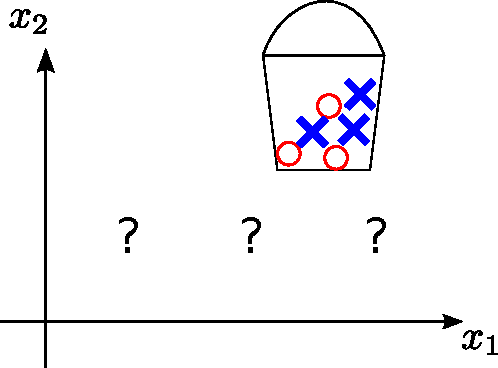
\includegraphics[width=0.7\textwidth]{img/shatter_arrangement_1}
	\notesonly{
	\captionof{figure}{A perceptron cannot always separate this arrangement.}
	}
\end{center}
\end{minipage}
\begin{minipage}{0.45\textwidth}
\begin{center}
	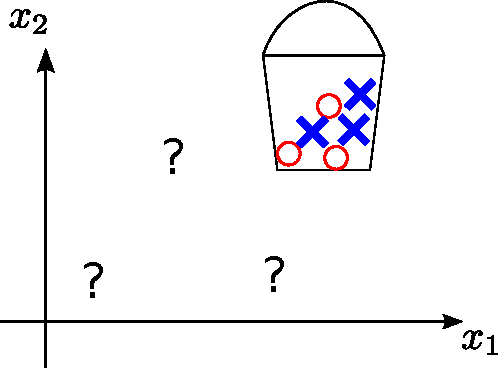
\includegraphics[width=0.7\textwidth]{img/shatter_arrangement_2}
	\notesonly{
	\captionof{figure}{A perceptron can always separate this arrangement.}
	}
\end{center}
\end{minipage}
	\notesonly{
	\captionof{figure}{An arrangement of 3 points in 2D.}
	}
\end{center}

\mode<article>{
It does not have to be able to for all possible arrangements (placements) of the $p$ points.
If there exists at least \textbf{one} dataset for which it can perfectly predict all label configurations, then the model shatters this.
}
\end{frame}

\begin{frame}\frametitle{\secname}


\mode<presentation>{
\begin{center}
	\includegraphics<1>[width=0.4\textwidth]{img/meme_vc_notdim}
\end{center}
}

\only<1>{
$\dvc$ is not actually a dimension but a single number \emph{capacity measure} 
of a model class that is parameterized by $\vec w$.\slidesonly{\\[5mm]}\notesonly{\\}
}

\underline{Definition}:\\

\only<1>{
$\dvc :=$ \underline{maximal number of data points $p$} that a model can \emph{shatter}.\\

}
\only<2>{
In other words, The VC dimension is the largest \# of points  
$p$ for which there exist at least one dataset  
$\vec X = \left(\vec x^{(1)}, \ldots, \vec x^{(p)}\right)^\top $ for which all  
$2^p$ label configurations can be solved with zero error.\\

}
\only<3>{
In more words: $\dvc$ is the \underline{maximal number of data points $p$} for which \emph{all} possible label configurations $\{y_{T}^{(\alpha)} \in \{-1,1\}\}_{\alpha=1}^{p}$ can be perfectly trained (i.e. $E^{T}_{[\vec w]} = R_{\text{emp}[\vec w]} = 0$) by tuning the model parameters $\vec w$.
If (at least) one dataset $\{(\vec x^{(\alpha)}, y_{T}^{(\alpha)})\}_{\alpha=1}^{p}$ with $p$ points exists such that the model can be tuned to perfectly classify any label configuration for that dataset, then the $\dvc$ for this model class is $p$.
}

\end{frame}

\begin{frame}

\mode<presentation>{
\begin{center}
\begin{minipage}{0.45\textwidth}
\begin{center}
	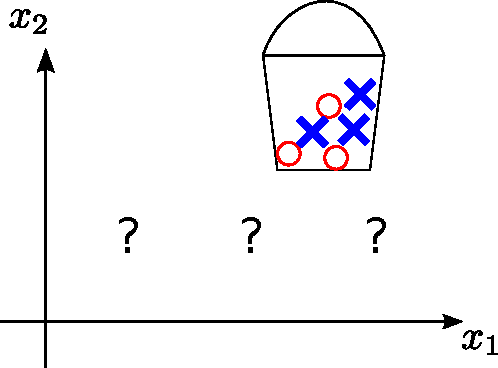
\includegraphics[width=0.7\textwidth]{img/shatter_arrangement_1}
	\notesonly{
	\captionof{figure}{A perceptron cannot always separate this arrangement.}
	}
\end{center}
\end{minipage}
\begin{minipage}{0.45\textwidth}
\begin{center}
	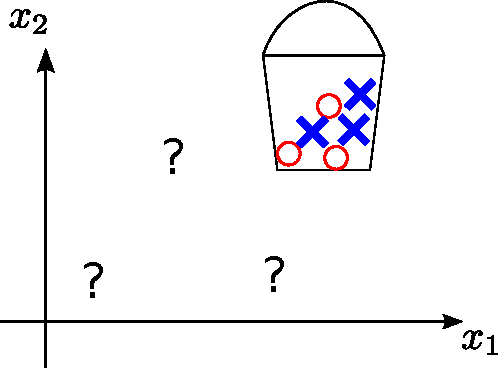
\includegraphics[width=0.7\textwidth]{img/shatter_arrangement_2}
	\notesonly{
	\captionof{figure}{A perceptron can always separate this arrangement.}
	}
\end{center}
\end{minipage}
	\notesonly{
	\captionof{figure}{An arrangement of 3 points in 2D.}
	}
\end{center}
}

\question{What was the $\dvc$ for our model in the previous example?}

\end{frame}

\begin{frame}

\underline{Examples}:

\begin{align}
&{\dvc}^{\text{perceptron}} &\kern-12ex=\;\;& N+1 = \text{\#params}\\
&{\dvc}^{\text{MLP}} &\kern-12ex=\;\;& \mathcal{O}(\text{\#params}^{2})\\
&{\dvc}^{k\text{NN}} &\kern-12ex=\;\;& \infty\\
&{\dvc}^{\text{sinusoid}} &\kern-12ex=\;\;& \infty
\end{align}

\begin{equation}
y^{\text{sinusoid}}(x;w) = \sign \big\lbrack \sin\left( w x \right) \big\rbrack    
\end{equation}

\pause

\question{How is ${\dvc}^{\text{sinusoid}} = \infty$? There's only 1 parameter!}

\mode<article>{
The parameters of the sinusoidal are amplitude, phase and frequency. A total of 3 parameters. Regardless of how many points there are, it is always possible to find values for the 3 parameters such that the sinusoidal goes through all $p$ points.
}
    
\end{frame}

